% Requires:
% \providecommand{\glsxtrshort}[1]{#1}
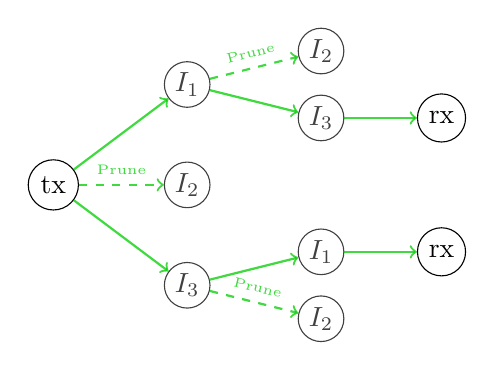
\begin{tikzpicture}[
    scale=0.85,
    % --- Styles ---
    % Tree Styles
    tree_node/.style={draw, circle, opacity=0.75, inner sep=0pt, text width=5mm, align=center},
    tree_root/.style={tree_node, inner sep=1pt,opacity=1},
    tree_leaf/.style={tree_root},
    edge_valid/.style={->, draw=green!80!black, thick, opacity=0.75},
    edge_valid_2/.style={edge_valid},
    edge_invalid/.style={edge_valid, dashed},
    prune_label/.style={midway, above, sloped, font=\tiny, text=green!80!black, opacity=0.75}
  ]
  % Level 0
  \node[tree_root] (T0) at (0,0) {\glsxtrshort{tx}};

  % Level 1
  \node[tree_node] (T1) at (2.0, 1.5) {$I_1$}; % Leads to Path 1
  \node[tree_node] (T2) at (2.0, 0) {$I_2$};   % Invalid (Prune)
  \node[tree_node] (T3) at (2.0, -1.5) {$I_3$}; % Leads to Path 2

  % Edges L0 -> L1
  \draw[edge_valid] (T0) -- (T1);
  \draw[edge_invalid] (T0) -- (T2) node[prune_label] {Prune};
  \draw[edge_valid_2] (T0) -- (T3);

  % --- Branch 1: TX -> o1 -> o3 ---
  \node[tree_node] (T11) at (4.0, 2.0) {$I_2$}; % Prune
  \node[tree_node] (T12) at (4.0, 1.0) {$I_3$}; % Valid
  \draw[edge_invalid] (T1) -- (T11) node[prune_label] {Prune};
  \draw[edge_valid] (T1) -- (T12);
  % Leaf
  \node[tree_leaf] (T12R) at (5.8, 1.0) {\glsxtrshort{rx}};
  \draw[edge_valid] (T12) -- (T12R);

  % --- Branch 2: TX -> o3 -> o1 ---
  \node[tree_node] (T31) at (4.0, -1.0) {$I_1$}; % Valid (Changed from o2 to o1)
  \node[tree_node] (T32) at (4.0, -2.0) {$I_2$}; % Prune
  \draw[edge_valid_2] (T3) -- (T31);
  \draw[edge_invalid] (T3) -- (T32) node[prune_label] {Prune};
  % Leaf
  \node[tree_leaf] (T31R) at (5.8, -1.0) {\glsxtrshort{rx}};
  \draw[edge_valid_2] (T31) -- (T31R);

\end{tikzpicture}
